\documentclass[12pt, a4paper,titlepage]{article}
\usepackage{ae}
\usepackage{lmodern}
\usepackage{amsfonts}
\usepackage{amsmath}
\usepackage{amssymb}
\numberwithin{equation}{section}
\numberwithin{figure}{section}
\usepackage{epsf}
\usepackage{epsfig}
\usepackage{graphicx}
%\usepackage[margin=2cm]{geometry}
\usepackage[T1]{fontenc}
\usepackage[english]{babel}

%\usepackage{showkeys}
\usepackage{setspace}
\frenchspacing
\linespread{1.3}
\usepackage{indentfirst}
\usepackage[utf8]{inputenc}
\usepackage{float}

\usepackage{wrapfig}
\usepackage{subfig}
\usepackage{multirow}
\usepackage{array}
\usepackage{tabularx}
\usepackage[calcwidth]{titlesec}
\usepackage{calc}

\usepackage{geometry}
%kotesre
\geometry{left=2.5cm,right=1.5cm,top=2.0cm,bottom=2.0cm}
%standard
%\geometry{left=2.0cm,right=2.0cm,top=2.0cm,bottom=2.0cm}

\newcommand*{\Resize}[2]{\resizebox{#1}{!}{$#2$}}%


\usepackage[pdftex]{hyperref}
	\hypersetup{colorlinks=true,
		pdfstartview=FitV,
		linkcolor=black,
		unicode=true,
		citecolor=black,
		urlcolor=black
		pdfauthor={Galgóczi Gábor, galgoczi.gabor@wigner.mta.hu},
		pdfsubject={TDK dolgozat},
		pdftitle={}
	}
	
	%\usepackage{biblatex}

%\usepackage[dvips]{graphicx}
%\usepackage{ucs}
%\usepackage[latin2]{inputenc}
%\usepackage{t1enc}
%\def\magyarOptions{defaults=prettiest}
%\usepackage[magyar]{babel}
%\usepackage{fontenc}
%\usepackage{graphicx}
%\usepackage{float}
%\usepackage{textcomp}
%\usepackage{array}
%\usepackage{tabularx}
%\usepackage{booktabs}
%\usepackage{color}
%\usepackage{ae}
%\usepackage{lmodern}
%\usepackage[margin=2 cm]{geometry}
%\usepackage{wrapfig}
%\usepackage{subfig}
%\usepackage{multirow}

\newcommand{\red}[1]{\textbf{\textcolor{red}{#1}}}
\newcommand{\pink}[1]{\textbf{\textcolor{magenta}{#1}}}
\newcommand{\blue}[1]{\textbf{\textcolor{blue}{#1}}}
\newcommand{\green}[1]{\textbf{\textcolor{green}{#1}}}
\usepackage[none]{hyphenat}
\sloppy
\titleformat{\section}{\large \bf }{\thesection.}{.5 em}{}[\vspace{-0.8 em}\rule{\titlewidth}{1pt}]


\begin{document}

\begin{titlepage}

\begin{center}
\ \\

\vspace{1 cm}
\begin{large}\textbf{Detailed feasibility study of a gamma ray detector system for nanosatellites using GEANT4 simulations}\end{large}\\
\vspace{1 cm}
%\begin{larger}\textbf{BSc szakdolgozat}\\ \end{larger}
%\vspace{0.5 cm}
\textit{\textbf{Galgóczi Gábor$^{*}$, Fizikus MSc szak, 2. évfolyam}}\\
Eötvös Loránd Tudományegyetem, Természettudományi Kar\\
WIGNER Fizikai Kutatóközpont - MTA\\
\vspace{1.5cm}
\begin{figure}[H]
\centering
\begin{tabular}{ >{\centering\arraybackslash}m{2in}  >{\centering\arraybackslash}m{2.5in}  }


\includegraphics[width=53.0mm]{images/regard.jpg}
\end{tabular}
\end{figure}

\begin{figure}[H]
\centering
\begin{tabular}{ >{\centering\arraybackslash}m{2in}  >{\centering\arraybackslash}m{2.5in}  }


\includegraphics[width=45.0mm]{images/elte.png} \parbox{0pt}{\rule{0pt}{2ex+\baselineskip}} &
\hspace{0.2 cm}

\includegraphics[width=40.0mm]{images/wigner.png}
\end{tabular}
\end{figure}


%\begin{figure}
%\centering
%\begin{subfigure}{5\textwidth}
 % \centering
  %\includegraphics[width=4\linewidth]{bme_logo_kicsi.jpg}
%\end{subfigure}%
%\begin{subfigure}{5\textwidth}
 % \centering
  %\includegraphics[width=4\linewidth]{image.jpg}
%\end{subfigure}
%\end{figure}



\vspace{0.1 cm}
\end{center}

\begin{center}
\begin{tabular}{ll}
\centerline{ Témavezetők: } \\
\centerline{ Conseil Européen pour la Recherche Nucléaire (CERN)}
\end{tabular}
\end{center}
\begin{center}

\vspace{2.5 cm}
\large \textbf {2016}\\
\end{center}
\end{titlepage}
%\doublespacing
\tableofcontents
%\singlespacing
\pagenumbering{roman}



\pagebreak
\pagenumbering{arabic}
\setcounter{page}{1}



%%%%%%%%%%%%%%%%%%%%%%%%%%%%%%%%%%%%%%%%

\section{Introduction}

High energy astrophysics

\subsection{Aim of the simulation}

The main aim of the paper, therefore this thesis is to optimize the scintillators of the CubeSats (miniaturized satellites) in the Constellation Gamma satellites. The second aim is to understand how the material of the CubeSat would affect the gamma photons that the satellite is meant to detect.

\subsection{The Constellation Gamma (ConGa) fleet}

\subsection{The simulated setup}


HAMAMATSU S13360-6050CS

datasheet of QE:
%http://www.hamamatsu.com/resources/pdf/ssd/s13360_series_kapd1052e.pdf

esr foil:
Please check "ESR from 3M" company. e.g.,
%http://multimedia.3m.com/mws/media/466120O/esr.pdf

\subsection{Simulation}

In order to understand how the $\gamma$ photons -- that the CubeSat is meant to detect -- interact with the matter of the satellite simulations are needed. In a simulation it is also possible to determine the optimal geometry that would lead to the best GRB detection. 

The Geometry... XXX TRacking (Geant4) 

\subsection{Fine tuning the optical parameters}

Most relevant parameters:
\begin{itemize}
\item absoprtion length of the scintillator material
\item scintillation yield
\end{itemize}

\section{Setup}

Size of the scintillator is, the aluminium housing thickness is, the size of the SiPM is...

Parameters of the CsI(Tl) scintillator REF

\begin{itemize}
\item Scintillation yield (Number of photons produced by given keV depleted in the scintillator)
\item The energy spectra of the produced scintillation
\item The time constant of the scintillation photon creation
\item The absorbtion length of the optical photons
\item Birks constant?
\end{itemize}

Optical parameters of the materials and surfaces:
\begin{itemize}
\item Refractive indices of all relevant materials
\item Reflection
\item The detection efficiency of the SiPM detectors
\end{itemize}

\section{Results of the simulation}
\subsection{Comparison of the results of the simulation with experiments}

The cross section for photoeffect is far the largest by far for low energy gamma photons.
The ionized nuclei and the secondary electrons generates scintillation.

ADC / energy calibration from measurement 20170829

illetve az egy chanellel: grb\_status3 

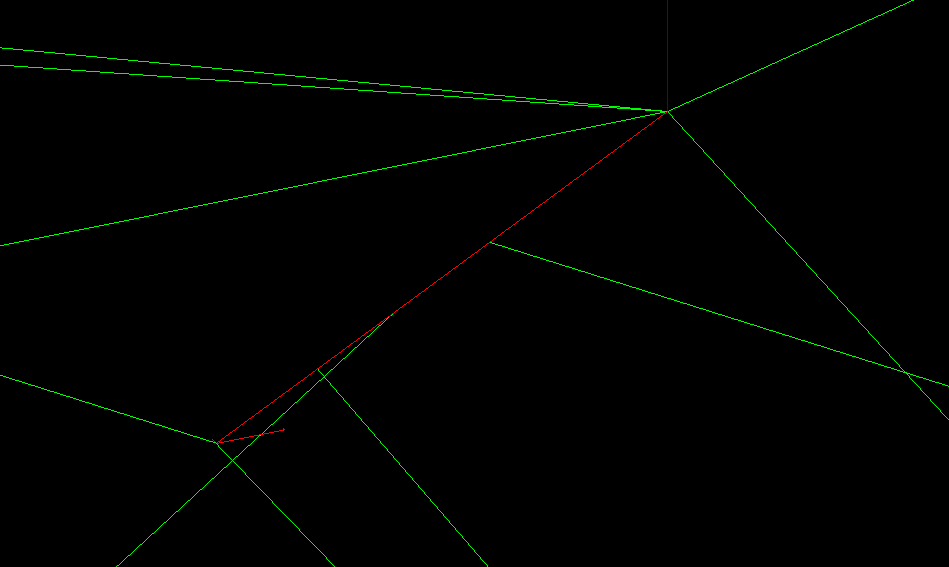
\includegraphics[width=130.0mm]{images/secondary.png}


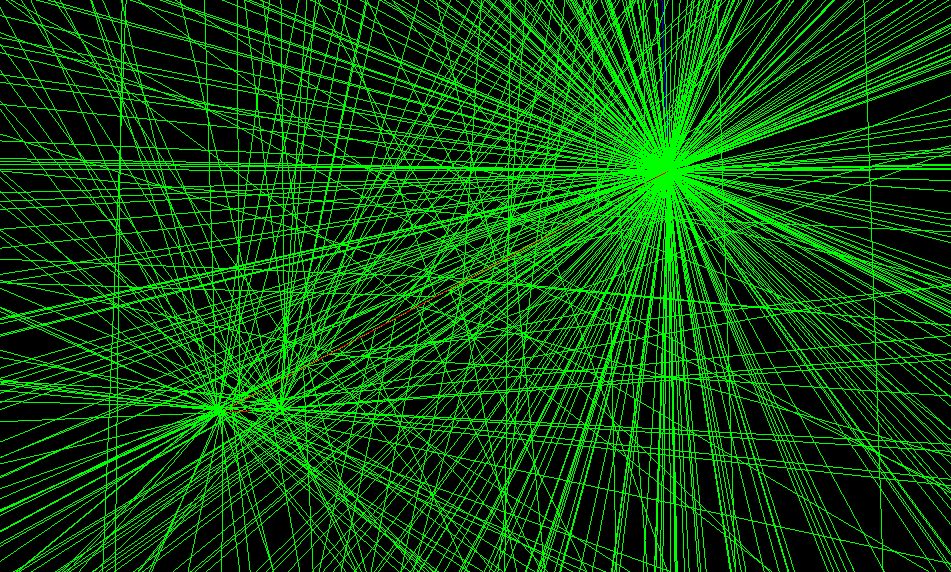
\includegraphics[width=130.0mm]{images/secondary2.png}

Also the nuclei that is ionized by the gamma produces photons.

\subsection{X-ray fluorescence}
Histogram without fluorescence, turned out in LXeEMPhysics line 140-159

Histogram with flo

\subsection{Simulation of background in space}


\subsection{Optimalization of the scintillator detectors}
\section{Conclusion}

\section{Acknowledgment}

 
\pagebreak

\addcontentsline{toc}{section}{References}
\begin{thebibliography}{99}
\interlinepenalty=10000

\bibitem{tgemadv} C. Shalem, R. Chechik, et al.,\\
Advances in Thick GEM-like gaseous electron multipliers—Part I: atmospheric pressure operation,\\
Nuclear Instruments and Methods in Physics Research A, vol. 558, page 475-489, 2006

\end{thebibliography}

\pagebreak




\end{document}

\begin{figure}[h!]
\centerline{
\includegraphics[width=260pt,angle=0]{images/let_setup.png}}
\caption{Az általam használt OTPC a gázrendszerével, illetve a kiolvasórendszerével együtt}
\end{figure}

Sötét anyag kutatásra jó beveztő:
https://arxiv.org/pdf/1510.02170.pdf
Nuclear physics:
https://indico.fnal.gov/conferenceDisplay.py/abstractBook?confId=8976

%%%%%%%%%%%%%%%
Alkalmazások


M. Pomorski, M. Pfutzner
M. Pomorski et al. Phys. Rev. C 90, 014311 (2014)

Micromegas-os kiolvasás J. B. R. Battat, Nucl. Instr. Meth. A 755(2014)6.

[grid???] U. Titt, V. Dagendorf et al., (Nucl. Instr. Meth. A 477 (2002) 536:	 
grids, pure TEA at low pressure, (electron counting / nano-dosimetry)

%%%%%%%%%%%%%%

Performance of an optical readout GEM-based TPC, L.M.S. Margato a...

optikai úton kiolvasott tpc-k: florian e-mailjéből

LET TPC

radon és polónium energiáira cikkek